\documentclass{report}

\usepackage{../../../../../LaTeX/marzstyle}

%\runningheads{Privacy and Data Security}{Exercise 01}

\fancyhead[L]{
	\begin{tabular}{l}
		\LARGE \textbf{\textsc{Concurrency}} \\
		\large Exercise 02
	\end{tabular}
}
\fancyhead[R]{
	\begin{tabular}{r}
		Marcel Zauder 16-124-836 \\
		Pascal Gerig 16-104-721
	\end{tabular}
}

\setcounter{chapter}{2}

\begin{document}
	\section{Several Questions}
	\startsection
		\begin{enumerate}[a)]
			\item \textit{What states can a Java thread be in?} \\
			A thread can be either \textsc{new}, when the thread is created but has not yet started, \textsc{runnable}, thread is executed in the Java Virtual Machine, \textsc{blocked}, a thread that is waiting, i.e. for a monitor lock to be released, \textsc{waiting}, a thread that waits indefinitely for another thread to finish its task, \textsc{timed-waiting}, a thread is waiting for a specified amount of time, and \textsc{terminated}, a thread that has exited. At one point a thread can only be in one of those states. 
			\item \textit{How can you turn a Java class into a monitor?} \\
			Each object in Java can be a monitor. For this its public methods must all be synchronized such that the access to this particular object is mutually exclusive.
			\item \textit{What is the Runnable interface good for?} \\
			A thread can be instantiated using a Runnable interface, such that the class which specifies the behaviour of the thread can inherit from another superclass which is not possible when already inheriting from the Thread class because Java only allows single inheritance.
			\item \textit{Specify an FSP that repeatedly performs hello, but can stop at any time.} \\
			The non-deterministic FSP would look like the following: \\
			HELLO = (hello -> HELLO | hello -> STOP).
		\end{enumerate}
	\closesection
	
	\section{Singleton}
	\startsection
		\begin{enumerate}[a)]
			\item If no singleton is there yet, then multiple threads can instanciate different singletons simultanously and return those.
			\item
			\begin{minted}{java}
public class Singleton {
	private static Singleton instance = null;
	private Singleton() {}
	public static synchronized Singleton getInstance() {
		if(instance == null) {
			instance = new Singleton();
		}
		return instance;
	}
}
			\end{minted}
			\item There is a bottleneck because only one thread can get the singleton instance at a certain moment. We can improve this, by only protecting the actual critical section instead of the entire method. In this case, we must guarantee that only one object is created, once that object is created, only accessing it is not critical, thus we can improve the code as follows, by only protecting the creation of the object:
			\begin{minted}{java}
public class Singleton {
	private static Singleton instance = null;
	private Singleton() {}
	public static Singleton getInstance() {
		if(instance == null) {
			synchronized(Singleton.class) {
				if(instance == null) {
					instance = new Singleton();
				}
			}
		}
		return instance;
	}
}
			\end{minted}
		\end{enumerate}
	\closesection
	
	\section{LTSA}
	\startsection
		\begin{enumerate}[a)]
			\item APPOINTMENT = (hello -> converse -> goodbye -> STOP).
			\item HOLIDAY = (arrive -> relax -> leave -> HOLIDAY).
			\item SPEED = (on -> ON), \\
			ON = (off -> SPEED | speed -> ON).
			\item LEFTONCE = (ahead -> INTERNALSTATE), \\
			INTERNALSTATE = (right -> LEFTONCE | left -> STOP).
			\item TREBLE = (in[n:1..3] -> out[n*3] -> TREBLE).
			\item const COUNTER = 5 \\
			FIVETICK  = TICK[1], \\
			TICK[n:1..COUNTER] = (when (n<COUNTER) tick -> TICK[n+1] \\
			| when (n==COUNTER) tick -> STOP).
			\item PERSON = (workday -> WORKDAY | holiday -> HOLIDAY), \\
			WORKDAY = (sleep -> work -> PERSON), \\
			HOLIDAY = (sleep -> SLEEPHOLIDAY), \\
			SLEEPHOLIDAY = (play -> PERSON | shop -> PERSON).

		\end{enumerate}
	\closesection
	
	\section{Race5K FSP}
	\startsection
		\begin{enumerate}[a)]
			\item \textit{How many states and how many possible traces occur if the number of steps is 5 (as in the lecture)?} \\
			Because we have 5 steps each competitor would have 6 states. Therefore we would get $6*6 \ = \ 36$ different states and a total of $\binom{10}{5} \ = \ \frac{10!}{5!(10-5)!} \ = \ 252$ traces.
			\item \textit{What is the number of states and traces for the generalized case (i.e., for n steps)?} \\
			The number of states would be $(n+1)^2$ and the number of traces is $\binom{2n}{n}$.
			\item \textit{Check your solution using the LTSA tool.} \\
			\begin{adjustwidth}{-6em}{}
				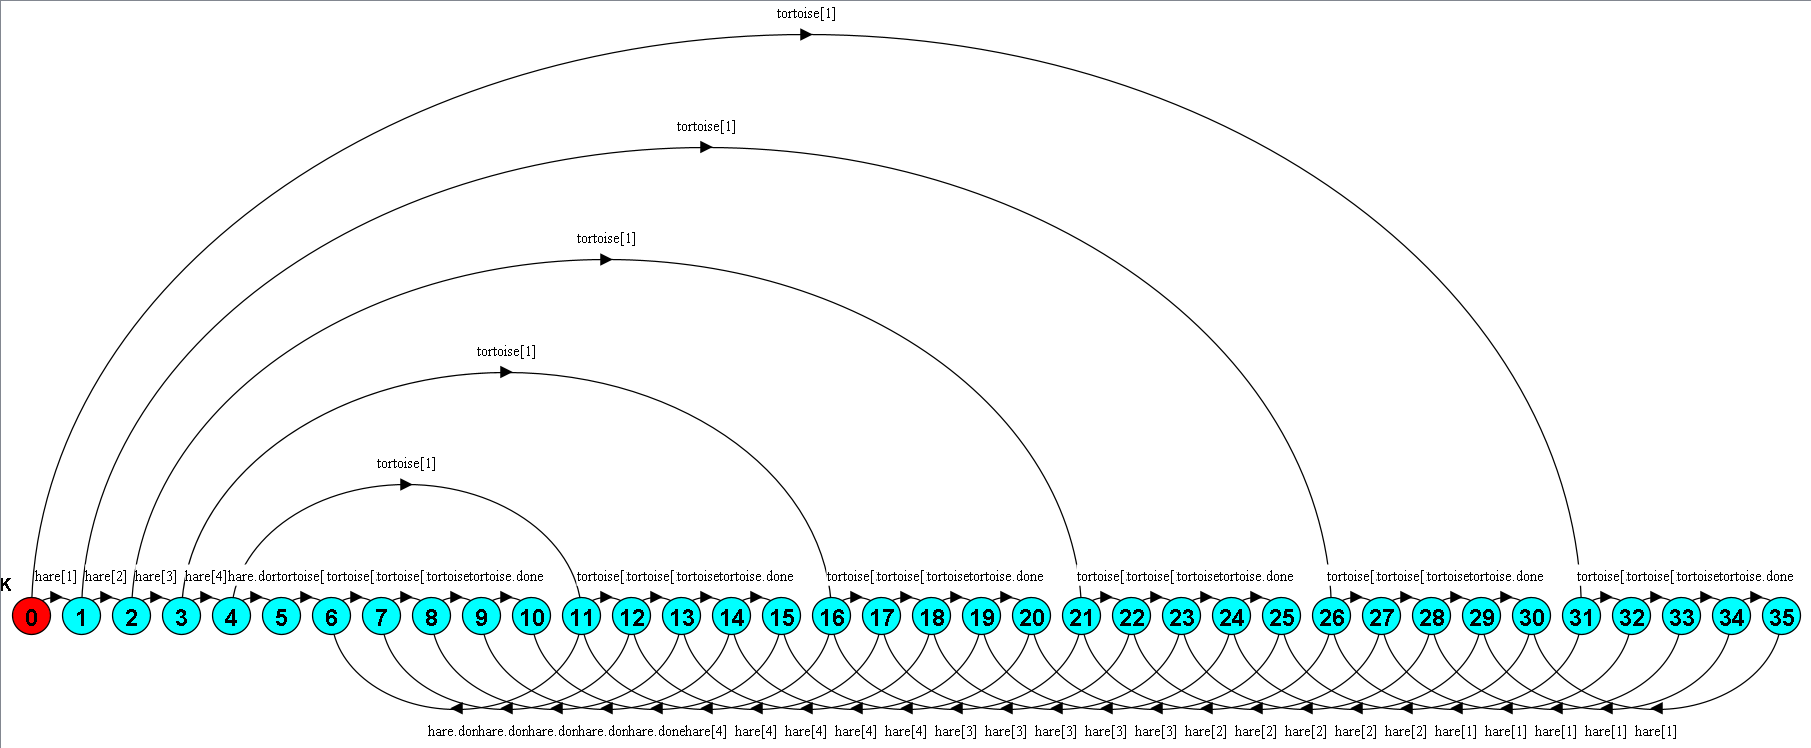
\includegraphics[scale=0.5]{Race5K.png}
			\end{adjustwidth}
		\end{enumerate}
	\closesection
\end{document}